\begin{figure}[H]
    \centering
    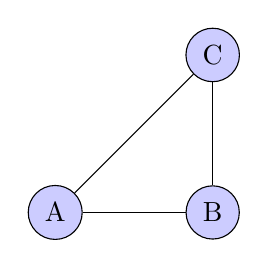
\begin{tikzpicture}
        \node[circle, draw, fill=blue!20] (A) at (0,0) {A};
        \node[circle, draw, fill=blue!20] (B) at (2,0) {B};
        \node[circle, draw, fill=blue!20] (C) at (2,2) {C};
        \draw (A) -- (B);
        \draw (B) -- (C);
        \draw (C) -- (A);
    \end{tikzpicture}
    \caption{Undirected graph example.}
    \label{fig:undirected-graph}
\end{figure}